\documentclass{svproc}
\usepackage{url}
\usepackage[options]{natbib}
\usepackage[hidelinks]{hyperref}
\usepackage{graphicx}
\usepackage{hyperref}


\graphicspath{ {./graphs/} }

\def\UrlFont{\rmfamily}

\begin{document}
\mainmatter
\title{Comparison of Classification Methods for Sentiment Analysis}
\subtitle{CS7IS2 Project (2020/2021)}
\author{Hannah Craddock \and Philippa Gilsenan \and Igor Ershov}

\institute{
\email{craddoch@tcd.ie}, \email{pgilsena@tcd.ie}, \email{ershovi@tcd.ie}}

\maketitle              % typeset the title of the contribution

\begin{abstract}
Sentiment analysis is a sub-field of natural language processing (NLP) and is the process of classifying opinions expressed in a piece of text be it positive or negative. This study involves the comparison of three classifier models via their ability to classify the sentiment of Amazon reviews. The resurgence of deep neural networks (DNNs) has revolutionised the field of NLP and sentiment analysis. Recurrent neural networks (RNNs), and specifically long short-term memory networks (LSTM), were once the go-to DNN for NLP applications, however a breakthrough development came in 2017 with the conception of the Transformer model at Google. This then led to Google’s Bidirectional Encoder Representations from Transformers (BERT) model which was designed to pretrain deep bidirectional representations from unlabelled text, its architecture beating every NLP benchmark. In addition to the DNN models, more traditional classification algorithms have also been utilised to classify sentiment such as Naïve Bayes or k-Nearest Neighbors (kNN). Here we wanted to test the hypothesis that the BERT model is significantly better than earlier DNNs such as LSTMs or more traditional classifiers such as Naïve Bayes. We did this by performing sentiment analysis on labelled Amazon review data and comparing the models performance across metrics such as the ROC curve and accuracy. The BERT model was found to have the best predictive performance, however at the cost of a prohibitively slow training time. If the speed of model execution is favoured over small gains in accuracy, Naïve Bayes was found to be optimal.
\keywords{Sentiment Analysis, NLP, BERT, RNNs, Naïve Bayes}
\end{abstract}
%

\section{Introduction}
In this work we implement and compare three distinct methods of classification to predict the polarity of Amazon reviews. Polarity refers to whether the review left by the user is positive or negative. This process of deriving the meaning or opinion of a text is called sentiment analysis, or opinion mining. Sentiment analysis itself is a form of natural language processing (NLP), a branch of artificial intelligence. The objective of NLP is to ingest, analyse and understand human language.

There is a wealth of textual data across the internet that is not being fully utilised. Unlike numerical data provided by humans, this textual data is not as easily understood by computers. Manually mining all this data would be both time and labour intensive and cost-inefficient. However, the task of NLP is not as straightforward due to the nuances of human languages. For example, double negation and sarcasm. Sentiment analysis is gaining traction as its applications span many industries and fields. It has uses in analysing the news, stock prices, social media, and in the context of our project, customer reviews. Some prevalent examples include the analysis of social media to predict the outcomes of elections or votes such as Brexit, and the analysis of news to predict stock price fluctuations. 
Three distinct methods of classification were evaluated and their efficacy was compared. These approaches will be expanded in the coming sections. This paper is laid out as follows: section two provides a state of the art of sentiment analysis. Section three provides a more detailed explanation of the approaches chosen as well as a problem definition. In section four the three approaches are evaluated and compared, finally in section five a conclusion to our work is presented.
\\
\\
\textbf{Presentation:}
\url{https://tcdud-my.sharepoint.com/:v:/g/personal/ershovi_tcd_ie/Eb7R3Rn9TmZBlxcumrE8HtsBOflN6LHr7bvCElk3U65L0w?e=1oWKUx}
\\

\\

\section{Related Work}
To date sentiment analysis has been used to detect the sentiment of natural language in a wide variety of domains, from its use in financial forecasting \citep{li2020incorporating} to real-time detection in political debates \citep{tumasjan2010predicting}. The pioneering work in the field was carried out by Pang et al. \citep{pang2002thumbs} and Turney \citep{turney2002thumbs}. The former applied supervised machine learning to determine the polarity of movie reviews, while the latter used unsupervised learning to classify the sentiment of customer reviews.

As well as a wide range of domains, a wide range of models have been used to detect sentiment. These models range from the more traditional Machine Learning models such as Naïve Bayes to the state-of-the-art Transformer based models such as BERT and RoBERTa \citep{carvalho2020evaluation}. Our aim was to test a sample of this range and compare the efficacy of the more traditional models with the state-of-the-art. Therefore a Naïve-Bayes model, an LSTM-RNN model and a BERT model were chosen for the purposes of this investigation.

The resurgence of deep neural networks has revolutionised the field of NLP given their high performance and reduced requirement for engineered features \citep{yin2017comparative}. DNNs have achieved remarkable performance in sentence and document modelling. Much progress has been made using Convolutional neural networks (CNNs) and recurrent neural networks (RNNs), particularly long short-term memory (LSTM) RNNs and they have both been widely used to handle various NLP tasks. CNNs are suited to extracting position-invariant features while the LSTMs are engineered to model units in sequence \citep{yin2017comparative}. LSTMs have feedback connections meaning they can process not only single data points but also entire sequences of data \citep{gers1999learning}, tempering the problem of the vanishing gradient characteristic of the original RNN architecture. We chose to apply an LSTM model to the task of sentiment analysis given its inherent applicability to sequences such as text. However, LSTMs can still only handle sequences of 100s, not 1000s or 10,000s, something which the next set of models overcome by avoiding sequential processing.

The watershed moment came in 2017 with the seminal paper from Google Research on Transformers and Self Attention; “Attention is all you need” (\cite{vaswani2017attention}; 19,869 citations at the time of writing). A transformer makes use of encoders and decoders consisting of multi-head layers of self-attention. Its development led to Google’s equally influential BERT Bidirectional model (\cite{devlin2018bert}; 17,968 citations at time of writing), which has surpassed human performance on many tasks. The first and best-known ‘masked’ language model, its architecture beating every NLP benchmark, and is the one being used to revamp both Google Search and Microsoft Bing over the past year \citep{carvalho2020evaluation}. A Bidirectional or ‘masked’ language model, it predicts a word or sequence of words, with context on either side. Various modifications have been made to the original BERT model, for example RoBERTa (Robustly optimised BERT approach) \citep{liu2019roberta} which applies dynamic masking and has achieved state-of-art results putting it first on the leader board for sentiment analysis models (see Figure I). Here we investigated whether the new masked BERT models would provide a significant increase in performance over the older DNNs and it was applied to our sentiment analysis task.

In addition to DNNs, well-established classification algorithms such as Naïve Bayes, k-Nearest Neighbors (kNN) and Support Vector Machines (SVM) have also been utilised to classify sentiment. In \citep{lochter2016short}, a grid search was used to select the optimal model across a variety of classification algorithms, including Naïve Bayes and kNN, via their ability to classify datasets of tweets. We likewise chose to test a more traditional classifier model and compare its efficacy to that of the more complex DNNs. The Naïve Bayes algorithm was chosen for its speed and simplicity. \begin{figure}
  \centering
    \includegraphics[scale=0.6]{graphs/models_leaderboard.png}
    \caption{State-of-the-art Sentiment Analysis models - current leaderboard \citep{paperswithcode}}
\end{figure}

\section{Problem Definition and Algorithm}
User reviews are not only beneficial for potential customers but can also provide companies with important insights into their customer base. In order to determine the polarity of reviews on a large scale, sentiment analysis is performed by machine learning models. The problem involved determining the polarity of Amazon reviews, specifically whether they are positive or negative, using three distinct models, BERT, Na\"ive Bayes and RNN to ascertain which method had the highest efficacy.

The models were trained on one dataset and tested on another. Originally, the training dataset consisted of 1,800,000 reviews and the test dataset 200,000. However, they were reduced to 100,000 training reviews and 20,000 test reviews to reduce training time. The datasets were balanced, containing equal amounts of positive and negative reviews. Standardised preprocessing was implemented to ensure consistency across the model results. This included the removal of stopwords and non-alphabetical characters. There are two labels, positive (2) and negative (1) which were updated to 1 and 0 respectively to be compatible with the sklearn package.

\subsection{Na\"ive Bayes}
Na\"ive Bayes is a fast and simple probabilistic algorithm for supervised learning. It is primarily used for classification however, as a poor estimator, it is not suitable for regression. The algorithm is based on Bayes’ theorem and is considered as na\"ive, or strong, as it assumes that the value of a feature is independent to the values of other features. As correlations between the features are not considered, each feature independently contributes to the probability of a label.

There are multiple Na\"ive Bayes methods, the uses of which are differentiated depending on whether the data is discrete or categorial, balanced or imbalanced as well as how the data is distributed. There are two variants typically used for text classification, Multinomial and Bernoulli. Multinomial was chosen as it performs better than Bernoulli with large vocabulary sizes \cite{mbn_vs_bnb}.

The sklearn MultinomialNB model was used to implement the algorithm. A number of variations to the model setup were tested in order to arrive at the optimal model. To convert the review text into numerical feature vectors, two vectorizers were compared. The count vectorizer gets the frequency of the word in the document while the tf-idf vectorizer gets the term frequency-inverse document frequency which reduces the impact of common words. Due to the removal of stopwords and a large vocabulary, the tf-idf vectorizer did not positively impact the model. By default, the number of features is set as the number of words in the vocabulary. A range of vocabulary limits were tested but in the end the whole vocabulary was included as restricting it negatively impacted the performance results. The algorithm requires a finite list of possible classification labels which in this case were positive and negative.


\subsection{LSTM RNN}
A recurrent neural network (RNN) is a type of neural network where neurons develop connections over a temporal sequence, allowing the model to keep track of dependencies in the input data. This is achieved with an internal state, also called a short term memory. An issue with classical RNNs is that the gradients propagated in the temporal sequence start tending to zero in what is called the ``vanishing gradient problem". \\
Long short-term memory (LSTM) architectures, first proposed by \cite{Hochreiter1997}, offer a solution to this by allowing some gradients to flow without changes. This enables the model to store long term dependencies between inputs effectively. A further critical contribution was made in \cite{gers1999learning} in the form of a forget gate, enabling the model to reset its state.
Using LSTM to tackle NLP tasks had been popular during the 2010s as it allows model training to consider the context.

An LSTM layer is comprised of recurrently connected memory blocks, which are themselves made up of one more LSTM memory cells. An LSTM memory cell contains the cell and three gates: an input gate, an output gate, and a forget gate. The cell allows the neuron to store the information, while the gates regulate how it handles information flow. The latter is the only way the model will interact with the cell. The input gate chooses what information from the current step is relevant to add to the cell, the forget gate selects what information from previous steps is worth keeping in the cell, and the output gate defines what the next state should be.

The implementation of the LSTM model in this study is based on the TensorFlow Keras framework. To convert the features into numerical values, the Keras TextVectorizer was used.

The model was trained multiple times to tweak the various hyperparameters;  no limit on the vocabulary size was set as results showed a negative drop in accuracy when it was implemented. The maximum length of an input vector was instead set to 50 in order to capture most phrases while reducing the model's input size. The loss function chosen is \textit{BinaryCrossentropy} as the model's output would be a prediction between positive and negative values, and the optimiser chosen was Adam with a learning rate of 1e-5, which was cross-validated between the values of  [5e-4,1e-4,5e-5,1e-5,5e-6,1e-6].

\subsection{BERT}
Bidirectional Encoder Representations from Transformers (BERT) is a transformer-based model of bidirectional encoders \citep{devlin2018bert}. A state-of-the-art pre-trained model developed by Jacob Devlin and his colleagues at Google is widely used for NLP tasks such as Sentiment Analysis. BERT is designed to pre-train deep bidirectional representations from unlabeled text. It can then be fine-tuned with just one additional output layer to form state-of-the-art models for a wide range of tasks. In \citep{devlin2018bert} BERT was shown to outperform many task-specific architectures and achieved state-of-the-art performance for eleven NLP tasks including pushing the GLUE score to 80.5% (7.7% point absolute improvement) and MultiNLI accuracy to 86.7% (4.6% absolute improvement).

As the name suggests, the BERT model uses a bi-directional transformer. The original Transformer design using Multi-Headed Self-Attention was proposed by \cite{vaswani2017attention}. The transformer circumvents the use of RNNs making use of encoders and decoders with multi-head layers of self-attention. Each Encoder has a separate feed-forward layer and a Self-Attention layer. For each input word, the Encoder generates query, value, and key vectors to produce a significance score for each word. In Multi-Headed Attention, each of the Attention blocks maintains its own encoder-generated query, value, and key vectors as well as separate Attention scores. The final score vector is generated by concatenating and multiplying the scores with a score matrix and loading it into a feed-forward network.

The bi-directional transformer in BERT was designed to pre-train deep bidirectional representations to extract context-aware features from the input text \citep{devlin2018bert}. BERT is trained on a sequence in both the forward and reverse direction, ensuring that the model captures the context of words in both directions. It is made up of 12 stacked transformer-encoder blocks, each of which has a multi-headed self-attention layer within it. The standard BERT-based model consists of a token vocabulary count of 30,000 words. This bidirectional model can capture the context of the data by linking all the tokens to the whole sequence in all the layers. Three distinct embeddings are created per token in the input sequence before the input is passed to the model. BERT provides a predefined tokenizer, \textit{BertTokenizer}, as used in this implementation. It is specific to the BERT model which creates the embedding sequences after pre-processing. Only the output layers are trained for specific data and are selected depending upon the type of task needed to be performed.

In this study, the BERT model pipeline was implemented using PyTorch and the BERT modules from the Transformers package. The specific BERT class is \textit{BertForSequenceClassification}. Like the RNN model an Adam Optimiser was chosen, with a learning rate of 2e-5 found to be optimal.


\section{Experimental Results}

During the evaluation, we will use the following metrics:
\begin{itemize}
    \item \textbf{Precision} - Precision is the fraction of correctly classified observations amongst all classified observations.
    \item \textbf{Recall} - Recall is the fraction of the total amount of actual positive cases that the model identifies correctly.
    \item \textbf{F1 score} - F1 score is a combination of precision and recall. It estimates the influence of false positives and false negatives.
    \item \textbf{Accuracy} - It is the number of correct predictions made by the model as a fraction of the total number of predictions
    \item \textbf{Confusion Matrix} - It is a quantitative way to visualize the performance that indicates the possible prediction outcomes.
    \item \textbf{ROC/AUC}  - The ROC curve corresponds to the True Positives rate plot against the False Positives rate; the curve will tend to reach the top left corner, the more the predictions it makes are correct.  The Area Under Curve is the graph's area under the ROC curve, a perfect value is 1.0, and the worst value is 0.
\end{itemize}

A test dataset of 20k reviews was used to evaluate our models, selected from a larger test dataset of 200k reviews. An equal number of positive and negative reviews is also present in the sampled test dataset. Two baselines were used for evaluation. A baseline that predicted the most frequent output (MF Baseline), and a simple Logistic Regression model trained with the features tokenized by CountVectorizer (T Baseline), with an L2 penalty and a value of C = 0.1 chosen using cross-validation.

\begin{table}[hbt!]
    \caption{Comparison of multiple metrics across models}
    \makebox[\linewidth]{
\begin{tabular}{|c|c|c|c|c|c|}
\hline
                    & MF Baseline & T Baseline & Naïve Bayes & RNN LSTM   & BERT       \\ \hline
Positive Precision  & 0           & 0.88       & 0.84        & 0.80       & 0.87       \\ \hline
Negative Precision  & 1           & 0.85       & 0.83        & 0.88       & 0.87       \\ \hline
Positive Recall     & 0           & 0.86       & 0.82        & 0.87       & 0.86       \\ \hline
Negative Recall     & 0.5         & 0.87       & 0.85        & 0.82       & 0.87       \\ \hline
Positive F1-Score   & 0           & 0.87       & 0.83        & 0.83       & 0.87       \\ \hline
Negative F1-Score   & 0.67        & 0.86       & 0.84        & 0.85       & 0.87       \\ \hline
Accuracy            & 0.5         & 0.86       & 0.83        & 0.84       & 0.87       \\ \hline
AUC                 & 0.5         & 0.93       & 0.90        & 0.92       & 0.96       \\ \hline
Training Time       & X           & 30 seconds & 2 minutes   & 1 hour & 66.5 hours \\ \hline
Final Training Loss & X           & X          & X           & 0.22       & 0.0084     \\ \hline
\end{tabular}
}
\end{table}
\begin{table}[hbt!]
    \caption{Baseline confusion matrices}
    \makebox[\linewidth]{
    \begin{tabular}{c      c }
    \textbf{Trained} & \textbf{Most Frequent} \\
        \begin{tabular}{|c|c|c|}
            \hline
                          & Pred. N & Pred. P \\ \hline
            True N &  8524                  &  1247                  \\ \hline
            True P &  1476                  &  8753                  \\ \hline
        \end{tabular} &
        \begin{tabular}{|c|c|c|}
        \hline
                      & Pred. N & Pred. P \\ \hline
        True N &  10000                  &  10000                  \\ \hline
        True P &  0                  &  0                  \\ \hline
        \end{tabular}
    \end{tabular}
    }
\end{table} \begin{table}[hbt!]
    \caption{Models confusion matrices}
    \makebox[\linewidth]{
    \begin{tabular}{c c c }
    \textbf{Na\"ive Bayes} & \textbf{RNN} & \textbf{BERT} \\
        \begin{tabular}{|c|c|c|}
        \hline
                      & Pred. N & Pred. P \\ \hline
        True N & 8471                   &   1529                 \\ \hline
        True P  & 1788                   &   8212                 \\ \hline
        \end{tabular} &
        \begin{tabular}{|c|c|c|}
        \hline
                      & Pred. N & Pred. P \\ \hline
        True N &  8795                  & 1981                   \\ \hline
        True P &  1205                  & 8019                   \\ \hline
        \end{tabular} &
        \begin{tabular}{|c|c|c|}
        \hline
                     & Pred. N & Pred. P \\ \hline
        True N &   8810                 &  1270                  \\ \hline
        True P &    0.14                &   8573                 \\ \hline
        \end{tabular}
    \end{tabular}
    }
\end{table}
\newpage
\\
\textit{Results - Discussion}
\\ In this section the model results are considered and compared. The BERT model was found to have the best predictive performance across all models, however at the cost of a prohibitively slow training time.
\\
\begin{figure}
  \centering
    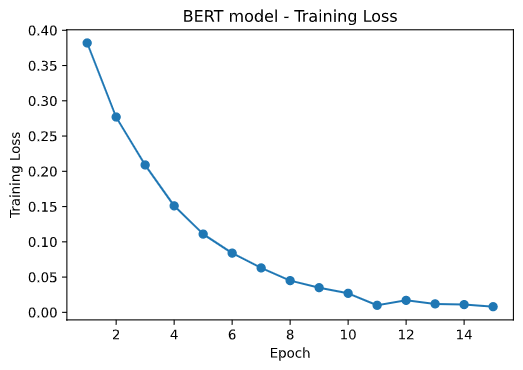
\includegraphics[scale=0.31]{BERT_loss.PNG}
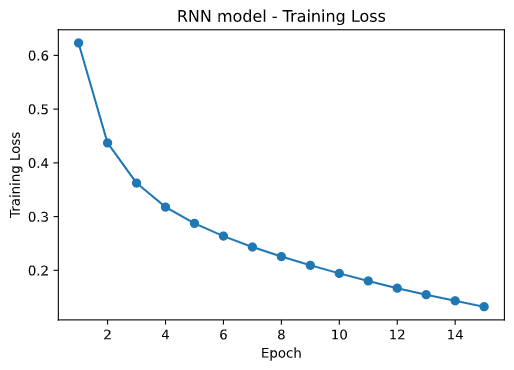
\includegraphics[scale=0.31]{RNN_loss.PNG}
    \caption{Loss plots of BERT and RNN models}
\end{figure}
\\
Overall, the performance is very good across the board. All trained models outperform the ``most frequent" baseline and have an AUC greater than 0.9. To put this in context, the most frequent baseline has an AUC of 0.5, while a perfect classifier would have an AUC of 1. The BERT Model achieves the highest AUC of 0.96, followed by the RNN model at 0.92 and the Naïve Bayes model at 0.90. Surprisingly, BERT is the only model that outperforms the trained baseline, while both the Naïve Bayes and RNN model score marginally worse.
\\
\begin{figure}
  \centering
    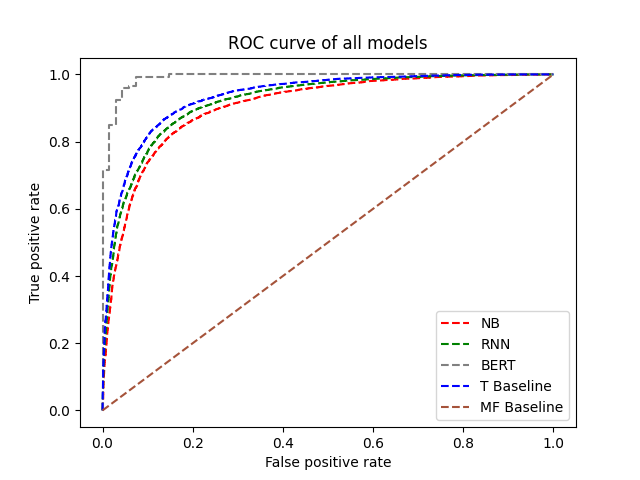
\includegraphics[scale=0.50]{ROC.PNG}
    \caption{ROC curves of all models}
\end{figure}
\\
The training times vary wildly. Both the baseline models and Naïve Bayes have low training times, which is expected due to their statistical nature. As expected, the two DNN models RNN and BERT, have slower training times as they are trained for multiple epochs. BERT in particular has a prohibitively slow training time, taking 66.5 hours to train, i.e. almost three days. BERT is however the brain-child of Google and has recently been used to revamp the companies' entire search engine. The standard BERT-based model consists of a token vocabulary count of 30,000 words and so this lengthy training period is perhaps unsurprising. Naturally Google has access to inordinate compute power and it is likely that they have optimised and parallelised their resources to enable rapid model training. If the speed of model execution is favoured over small gains in accuracy, the other models such as RNN or Naïve Bayes should be considered. However if model accuracy and performance is the priority, the BERT model is the winner.

\section{Conclusions}
In this work, three distinct methods of classification were implemented to predict the polarity of Amazon reviews. Across several domains, a wide range of models have been used to detect sentiment and our aim was to test a sample of this range and compare the efficacy of the more traditional models with the state-of-the-art. Accordingly a Naïve-Bayes model, an LSTM-RNN model and a BERT model were implemented and compared. BERT is a state-of-the-art pre-trained model that is beating every NLP benchmark and is the architecture being used to revamp both Google Search and Microsoft Bing engines. Here we tested the hypothesis that the BERT model is significantly better than earlier DNNs such as LSTMs or more traditional classifiers such as Naïve Bayes. We did this by performing sentiment analysis on labelled Amazon review data and comparing the models' performance across metrics such as the ROC curve and accuracy. The BERT model was found to have the best predictive performance, however at the cost of a prohibitively slow training time. Possible improvements to the training time could be made by optimising the computing approach. Graphics Processing Units (GPUs) can significantly accelerate the training process for deep learning models by taking advantage of a GPU's massively parallel architecture. Thus for future implementation of this study, the program could be designed to offload tasks to one or more GPUs potentially reducing the training time from days to hours. Despite it's simplicity, the Naïve-Bayes model had by far the superior training time, taking merely 2 minutes to train.  
Overall, if the speed of model execution is favoured over small gains in accuracy, Naive Bayes should be the chosen model over it's competitors. However if model accuracy and performance is the priority, the BERT model should be the default model of choice.

\bibliographystyle{apalike}
\bibliography{references.bib}

\end{document}
